\documentclass[12pt,a4paper,fleqn]{article}
\usepackage[utf8]{inputenc}
\usepackage{amssymb, amsmath, multicol}
\usepackage[russian]{babel}
\usepackage{graphicx}
\graphicspath{{pictures/}}
\DeclareGraphicsExtensions{.pdf,.png,.jpg}
\usepackage[shortcuts,cyremdash]{extdash}
\usepackage{wrapfig}
\usepackage{floatflt}
\usepackage{lipsum}
\usepackage{concmath}
\usepackage{euler}
\usepackage{tikz}  
\usetikzlibrary{graphs}

\oddsidemargin=-15.4mm
\textwidth=190mm
\headheight=-32.4mm
\textheight=277mm
\tolerance=100
\parindent=0pt
\parskip=8pt
\pagestyle{empty}
\renewcommand{\tg}{\mathop{\mathrm{tg}}\nolimits}
\renewcommand{\ctg}{\mathop{\mathrm{ctg}}\nolimits}
\renewcommand{\arctan}{\mathop{\mathrm{arctg}}\nolimits}
\newcommand{\divisible}{\mathop{\raisebox{-2pt}{\vdots}}}

\begin{document}
{\bf 1)} Обозначим: $N$~---~мн-во перестановок книг на поле, $\alpha_i$~---~св-во, означающее, что какие-то две из названных книг стоят рядом (таких свойств, соответственно три, для каждой возможной пары книг). \newline
$N(\overline{\alpha_1}, \overline{\alpha_2}, \overline{\alpha_3}) = N - C_3^1 \cdot N(\alpha_i) + C_3^2 \cdot N(\alpha_i, \alpha_j) - C_3^3 \cdot N(\alpha_1, \alpha_2, \alpha_3)$ \newline
\begin{itemize}
\item $N = 20!$ 
\item $N(\alpha_i) = 19 \cdot 2 \cdot 18!$ (выбираем два рядом стоящих места~---~$19$ вариантов, внутри этих двух местах книги можно переставить двумя способами, остальные книги~---~$18!$ способов расставить)
\item $N(\alpha_i, \alpha_j) = 18 \cdot 2 \cdot 17!$ (выбираем три места подряд~---~$18$ способов, внутри этих трех мест двумя способами можно переставить три книги (чтобы одновременно выполнялись выбранные условия), остальные книги переставляем $17!$ способами).
\end{itemize}
$N_0 = 20! - 6 \cdot 19! + 6 \cdot 18! = 272 \cdot 18!$ \newline
Ответ: $272 \cdot 18!$ \newline \newline
{\bf 2)} Обозначим: $N$~---~мн-во наборов по 7 карт, выбранных из колоды, $\alpha_i$~---~свойство, обозначающее отсутствие $i$-ой масти в колоде (масти пронумераем от 1 до 4). Тогда, по формуле включений и исключений: \newline
$N(\overline{\alpha_1},\overline{\alpha_2},\overline{\alpha_3},\overline{\alpha_4}) = N - C_4^1 \cdot N(\alpha_i) + C_4^2 \cdot N(\alpha_i, \alpha_j) - C_4^3 \cdot N(\alpha_i, \alpha_j,\alpha_k)$ (т.~к. для разных мастей и их сочетаний кол-во одно и то же, слагаемые обьединены по числу сочетаний, т.~е. $N(\alpha_i)$~---~кол-во наборов, в которых отсутствует $i$-я масть, таких мастей можно выбрать $C_4^1$. Для двух мастей~---~$C_4^2$ и т.~д. \newline
\begin{itemize}
\item $N = C_{36}^7$
\item $N(\alpha_i) = C_{27}^7$ (выбрасываем из колоды все карты одной масти и выбираем из них)
\item $N(\alpha_i, \alpha_j) = C_{18}^7$ (аналогично выбрасываем две масти из колоды)
\item $N(\alpha_i, \alpha_j, \alpha_k) = C_9^7$
\end{itemize}
Кроме того, $N(\overline{\alpha_1},\overline{\alpha_2},\overline{\alpha_3},\overline{\alpha_4})$~---~кол-во наборов, в которых есть все масти $\rightarrow$ \newline
$N(\overline{\alpha_1},\overline{\alpha_2},\overline{\alpha_3},\overline{\alpha_4}) = C_{36}^7 - 4 \cdot C_{27}^7 + 6 \cdot C_{18}^7 - 4 \cdot C_9^7$ \newline
Ответ:$C_{36}^7 - 4 \cdot C_{27}^7 + 6 \cdot C_{18}^7 - 4 \cdot C_9^7$ \newline \newline
{\bf 4)} $N$~---~мн-во функций алгебры логики, $\alpha_i$~---~свойство, означающее, что функция несущественно зависит от $i$-ой переменной. Тогда: \newline
$N(\overline{\alpha_1} \cdots) = 2^n - C_n^1 \cdot N(\alpha_i) + \cdots + (-1)^n \cdot N (\alpha_1, \alpha_2, \cdots)$ \newline
$N(\overline{\alpha_1} \cdots)$~---~искомое кол-во функций. \newline
$N(\alpha_i, \cdots$ = (для $k$ штук $\alpha$) $2^{n - k}$. Убираем указанные $k$ переменных, остается $n - k$, тогда функций для такого кол-ва переменных $2^{n - k}$. Тогда, чтобы получить необходимые функции, просто к каждому набору из $n - k$ допишем по $2^k$ наборов из $k$, причем значение функции остается одинаковым на одинаковых наборах из $n - k$. \newline
$N_0 = 2^n + \sum_{k = 1}^{n - 1} (-1)^k \cdot 2^{n - k} \cdot C_n^k + (-1)^n \cdot 2$ (последнне слагаемое в исходной сумме не подчиняется правилу $2^{n - k}$, т.~к. существует 2 функции, существенно не зависящие ни от какой из своих переменных~---~$0$ и $1$) \newline
Ответ: $2^n + \sum_{k = 1}^{n - 1} (-1)^k \cdot 2^{n - k} \cdot C_n^k + (-1)^n \cdot 2$ \newline \newline
{\bf 5)} Т.~. у любого художника готово как миниум $\dfrac{2}{3}$ картины, то, если предположить, что у каждого невыполненная область целиком лежит в области, которую выполнил другой, то пересечение их выполенных областей как миниум $\dfrac{1}{3} > \dfrac{1}{4}$, поэтому: \newline
Ответ: нет \newline \newline
{\bf 7)} Проведем дуги вокруг сферы по сторонам треугольника и разобьем его на 6 двуугольников: по 2 с углами $\alpha, \beta, \gamma$, причем три из них (с углами $\alpha, \beta, \gamma$) пересекаются дважды по искомой площади $x$ (с одного полюса и с другого), а трое других~---~не пересекаются вообще. (пояснения см. ниже)\newline
Площадь одного двухугольника с углом $\phi$ равна: $S_\phi = \dfrac{\phi}{2 \pi} \cdot S_0 = \dfrac{\phi \cdot 4\pi \cdot R^2}{2 \pi} = 2 \phi$ \newline
$S_0 = 4\pi = 2S_\alpha + 2S_\beta + 2S_\gamma - 4x$ \newline
$x = \alpha + \beta + \gamma - \pi$ \newline
Ответ: $x = \alpha + \beta + \gamma - \pi$ \newline \newline
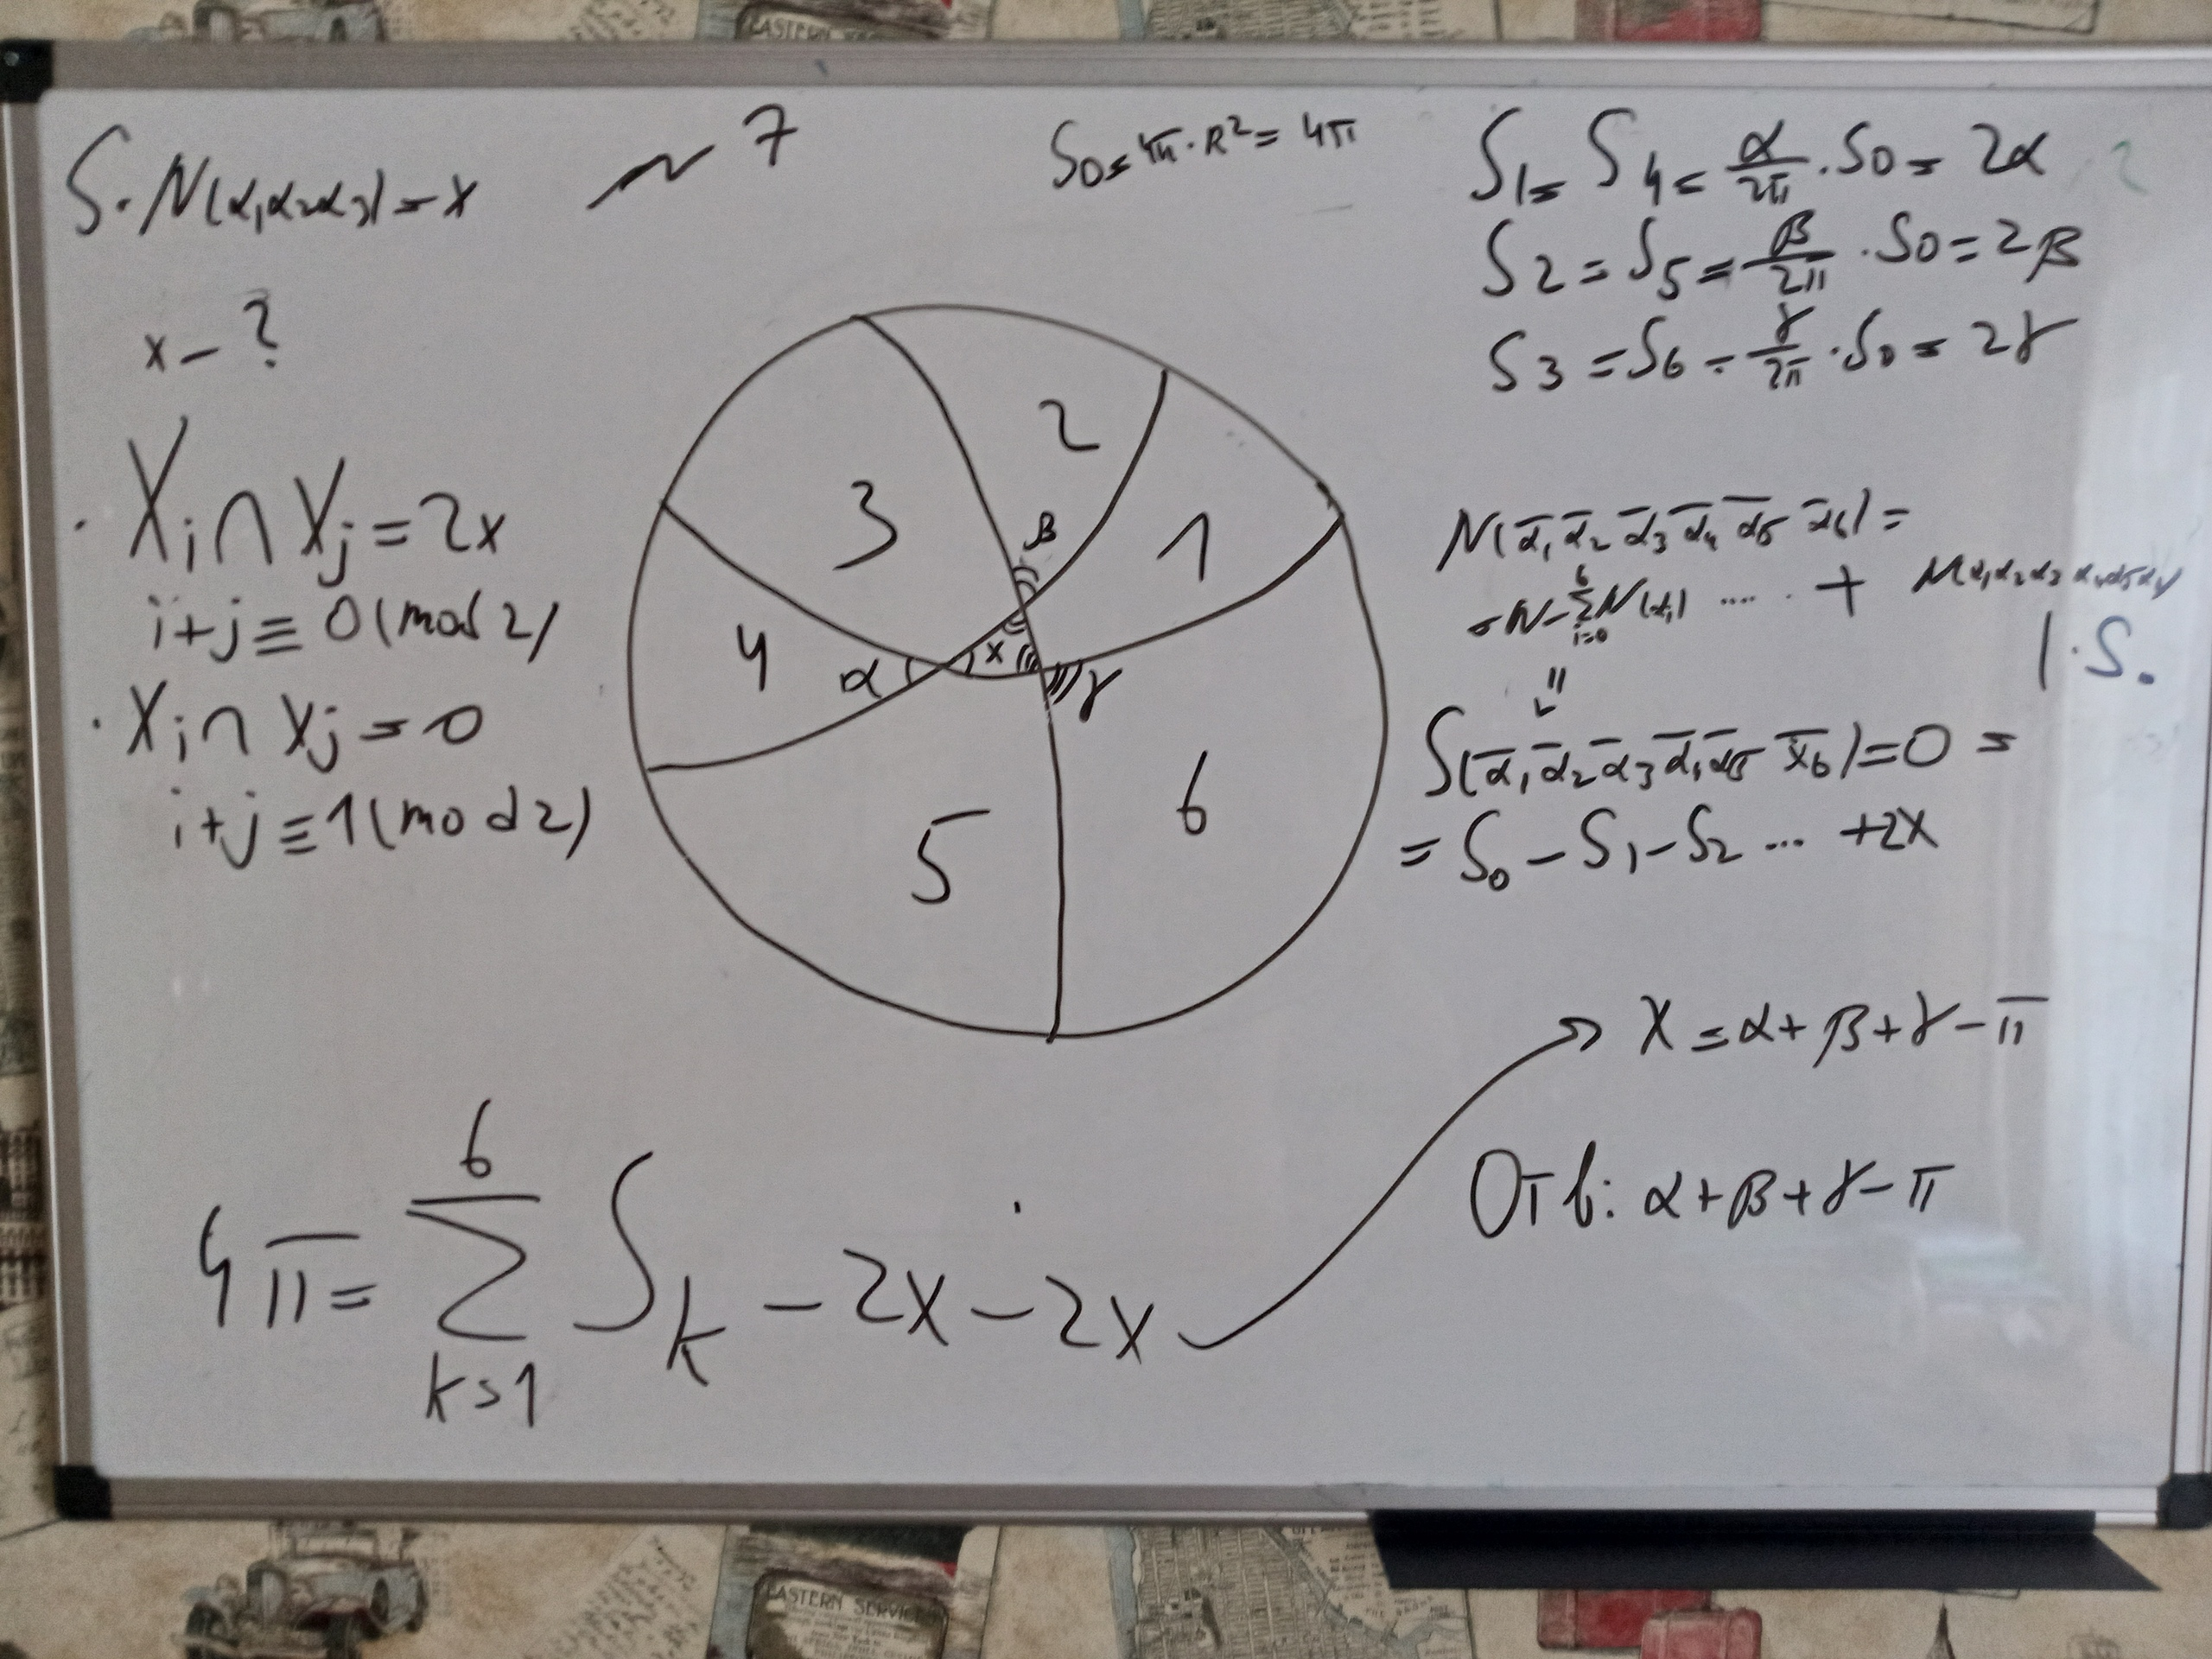
\includegraphics[scale=0.2]{ZKZU4eacRnk.jpg}
\end{document}